\documentclass[11pt, article]{amsart}

\usepackage{amsfonts}
\usepackage{amsmath}
\usepackage{amsthm}
\usepackage{amssymb}
\usepackage{esdiff}
\usepackage[utf8]{inputenc} % allow utf-8 input
\usepackage[T1]{fontenc}    % use 8-bit T1 fonts
\usepackage{hyperref}       % hyperlinks
\usepackage{url}            % simple URL typesetting
\usepackage{booktabs}       % professional-quality tables
\usepackage{amsfonts}       % blackboard math symbols
\usepackage{nicefrac}       % compact symbols for 1/2, etc.
\usepackage{microtype}      % microtypography
\usepackage{lipsum}
\usepackage{algorithm2e}
\usepackage{algpseudocode}
\usepackage{subfig}
\usepackage{siunitx}
\usepackage[pdftex]{graphicx}
\usepackage[all]{xy}

\def\vac{| \mathrm{vac} \rangle}

\begin{document}

\section{The multinomial ansatz}

We derive this ansatz by looking at the non-interacting Bose Hubbard model with $N$ particles in $M$ modes. In momentum space, its ground state is
%
\begin{equation}
  | \Phi \rangle = \frac{1}{\sqrt{N!}}{\left(\hat{c}^\dagger_0\right)}^N \vac\,,
\end{equation}
%
where $\hat{c}^\dagger_i$ is the momentum space creation operator. Applying the Fourier transform to the above equation yields
%
\begin{equation}
  | \Phi \rangle = \frac{1}{\sqrt{N!}}{\left[\frac{1}{\sqrt{M}}\sum_{i=1}^M \hat{a}^\dagger_i\right]}^N \vac\,,
\end{equation}
%
where $\hat{a}^\dagger_i$ is the real space creation operator. Using the multinomial theorem, this can be rewritten as
%
\begin{equation}\label{eq:multinomial}
  | \Phi \rangle = \frac{N!}{\sqrt{N!M^N}}
  \sum_{(\nu_i \in \mathbb{N}_0)_{i=1}^M, \sum_{i=1}^M\nu_i=N}
  \prod_{i=1}^{M}\frac{1}{\nu_i!}{\left(\hat{a}^\dagger_i\right)}^{\nu_i}\vac
\end{equation}
%
where the sum goes over all $M$-tuples of non-negative integers $(\nu_1, \nu_2, \dots, \nu_M)$, whose elements sum to $N$. We rewrite~\eqref{eq:multinomial} in terms of Fock states
%
\begin{equation}
  |f\rangle = |\nu_1, \nu_2, \dots, \nu_M\rangle = \prod_{i=1}^M\frac{1}{\sqrt{\nu_i!}}\left(\hat{a}_i^\dagger\right)\vac\,,
\end{equation}
%
yielding the final form of the ansatz
%
\begin{equation}\label{eq:multinomial-ansatz}
  |\Phi\rangle = \sqrt{\frac{N!}{M^N}}\sum_{|f\rangle}\left(\prod_{i=1}^{M}\frac{1}{\sqrt{\nu_i!}}\right)|f\rangle\,.
\end{equation}
%
For use with importance-sampled FCIQMC, it is useful to introduce a parameter $p$ to Eq.~\eqref{eq:multinomial-ansatz}:
%
\begin{equation}\label{eq:multinomial-ansatz-p}
|\Phi(p)\rangle =  \mathcal{N}\sum_{|f\rangle}\left(\prod_{i=1}^{M}\frac{1}{\nu_i!}\right)^p|f\rangle\,,
\end{equation}
%
where $\mathcal{N}$ is an unknown normalization constant. How the parameter affects the result is shown in Fig.~\ref{fig:example}.

\begin{figure}
  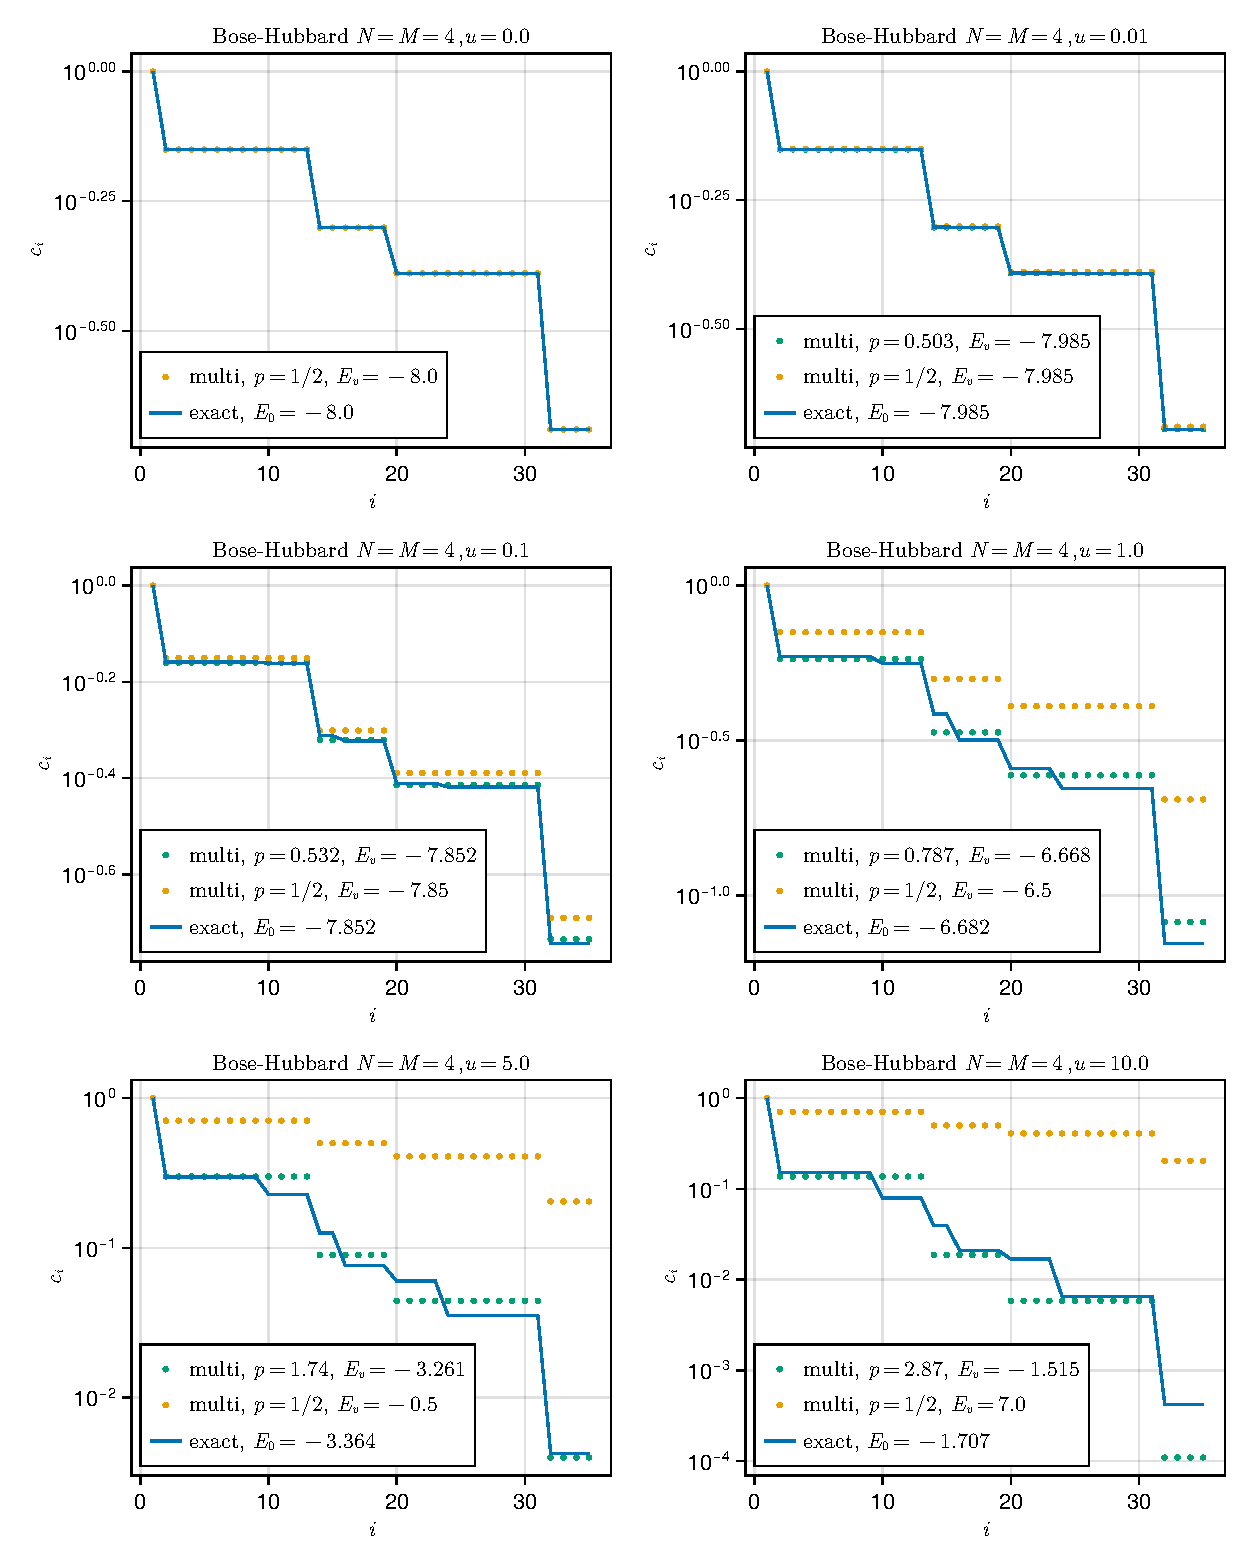
\includegraphics[width=\textwidth]{example}
  \caption{\label{fig:example}
    Comparison of the multinomial ansatz to the exact ground states of 1D Bose-Hubbard Hamiltonians with $N=4$ particles in $M=4$ sites and various interaction strengths $u$. The plot displays the coefficients of the true ground state eigenvector (labelled as exact), and the multinomial ansatz (Eq.~\eqref{eq:multinomial-ansatz-p}) with an optimal value of $p$, and with $p=1/2$ (as seen in Eq.~\eqref{eq:multinomial-ansatz}). The vector indices $i$ are ordered by the value of the ground state eigenvector.
  }
\end{figure}

\end{document}
